\documentclass[11pt]{article}
% Shared preamble for the notes in this repository. pdfLaTeX, TeX Live 2024 or later.
\usepackage[a4paper,margin=2.6cm]{geometry}
\usepackage[T1]{fontenc}
\usepackage{lmodern}
\usepackage{microtype}
\usepackage{amsmath,amssymb,amsthm}
\usepackage{graphicx}
\usepackage{booktabs}
\usepackage{enumitem}
\usepackage[dvipsnames]{xcolor}
\usepackage[hidelinks]{hyperref}
\hypersetup{colorlinks=true,linkcolor=MidnightBlue,citecolor=MidnightBlue,urlcolor=MidnightBlue}
\graphicspath{{../../figures/}}
\setlist{itemsep=2pt,topsep=4pt}

\newtheorem{theorem}{Theorem}
\newtheorem{proposition}[theorem]{Proposition}
\newtheorem{corollary}[theorem]{Corollary}
\newtheorem{conjecture}[theorem]{Conjecture}
\theoremstyle{definition}
\newtheorem{definition}[theorem]{Definition}
% Reusable derivations, numbered note.k; each note sets \notenumber. Indexed in DERIVATIONS.md.
\newcommand{\notenumber}{0}
\newtheorem{derivation}{Derivation}
\renewcommand{\thederivation}{\notenumber.\arabic{derivation}}
\newtheorem{question}{Question}
\theoremstyle{remark}
\newtheorem{remark}[theorem]{Remark}

\newcommand{\Z}{\mathbb{Z}}
\newcommand{\Q}{\mathbb{Q}}
\newcommand{\R}{\mathbb{R}}
\newcommand{\C}{\mathbb{C}}
\newcommand{\HH}{\mathbb{H}}
\newcommand{\SL}{\mathrm{SL}}
\newcommand{\Gal}{\mathrm{Gal}}
\newcommand{\Hom}{\mathrm{Hom}}
\newcommand{\repo}{\href{https://github.com/rmorleysmith/l-functions-and-physics}{\texttt{l-functions-and-physics}}}
\newcommand{\formal}{\href{https://github.com/rmorleysmith/morley-smith-formal}{\texttt{morley-smith-formal}}}
\newcommand{\script}[1]{\href{https://github.com/rmorleysmith/l-functions-and-physics/blob/main/scripts/#1}{\texttt{scripts/#1}}}
% A path inside the Lean repository; it may break after a slash.
\newcommand{\leanpath}[1]{\nolinkurl{#1}}

% Grades used in every status table.
\newcommand{\gradeLean}{\textsc{lean}}      % proved in Lean 4 with Mathlib
\newcommand{\gradeClassical}{\textsc{classical}}  % a published theorem, cited
\newcommand{\gradeComputed}{\textsc{computed}}    % checked numerically by a script in this repository
\newcommand{\gradeConvention}{\textsc{convention}}  % a choice of units or names
\newcommand{\gradeOpen}{\textsc{open}}      % a question, conjecture or working hypothesis
% The legend printed under every status table.
\newcommand{\gradelegend}{\par\nopagebreak\smallskip\noindent\begin{minipage}{\textwidth}\small
\gradeLean: proved in Lean 4 with Mathlib.
\gradeClassical: a published theorem.
\gradeComputed: checked numerically by a script in the repository \repo.
\gradeConvention: a choice of units or names.
\gradeOpen: a question, conjecture or working hypothesis.
\end{minipage}\par\medskip}
% A plain-language physical reading, placed after each derivation.
\newcommand{\physical}{\paragraph{In physical terms.}}


\title{The golden ratio: where it is, and where it is not}
\author{Richard Morley-Smith}
\date{Note 05 \quad November 2026}

\begin{document}
\maketitle

\begin{abstract}
\noindent
The symmetry of the twelve-tone circle is not the golden ratio.
It is the Klein four-group $\{1,5,7,11\}$ of note~01, and $\varphi = (1+\sqrt5)/2$ does not appear in it.
In fact $\varphi$ is the opposite kind of number.
Twelve-tone music exists because $\log_2(3/2)$ is unusually close to the fraction $7/12$, while $\varphi$ is the number worst approximated by fractions.
That is why plants use it: they need to avoid periodic arrangements.
The golden ratio does appear, precisely, in the modular world and in physics:
\begin{itemize}
\item the shortest closed geodesic on the modular surface has length $4\log\varphi$;
\item the modular curve $X(5)$ is an icosahedron, whose twelve vertices, the cusps, have coordinates in $\Q(\sqrt5)$;
\item the Ising chain in a magnetic field has a particle mass ratio $m_2/m_1 = \varphi$, predicted from $E_8$ and observed by neutron scattering.
\end{itemize}
We check each statement numerically and say where the evidence stops.
\end{abstract}

\section{Two kinds of number}

Every irrational $x$ has a continued fraction $[a_0;a_1,a_2,\dots]$.
Its convergents $p/q$ are its best rational approximations, and large partial quotients mean very good ones.
Hurwitz's theorem says that $q\,|qx-p| < 1/\sqrt5$ infinitely often for every irrational $x$, and that $\sqrt5$ cannot be improved.
The extreme case is $\varphi = [1;1,1,1,\dots]$, where $q\,|q\varphi - p|\to 1/\sqrt5 = 0.447$ at the convergents.
By contrast, $\log_2\frac32 = [0;1,1,2,2,3,1,5,2,23,\dots]$ gives $0.235$ already at $q=12$.
The script \script{golden\_ratio.py} checks both.

So the two numbers do opposite jobs.
Twelve-tone equal temperament works because one fraction, $7/12$, approximates the fifth well (note~01).
The golden ratio is the number that no fraction approximates well.

\section{Phyllotaxis}

Place seeds one by one at a fixed angle $\alpha$ of a turn and at radius $\sqrt n$ (Vogel's model).
\begin{itemize}
\item With $\alpha = 7/12$ the seeds fall on exactly twelve rays.
\item With the pure fifth $\alpha=\log_2\frac32$ they form twelve slowly curving arms.
\item With the golden angle $\alpha = 1/\varphi^2$ ($137.508^\circ$) they fill the disc evenly (Figure~\ref{fig:phyllo}).
\end{itemize}
By the three-gap theorem, the first $n$ points of any rotation divide the circle into gaps of at most three lengths.
For the golden angle, the ratio of the largest gap to the smallest never exceeds $\varphi^2 = 2.618$ for $20\le n\le 800$.
For the fifth it reaches $24.4$.
Douady and Couder reproduced the golden angle in a physical experiment with magnetised drops \cite{DouadyCouder}.
It emerges when each new element is placed as far as possible from the previous ones, a system that avoids periodic order.
This is the best-established case of $\varphi$ in nature.

\begin{figure}[ht]
  \centering
  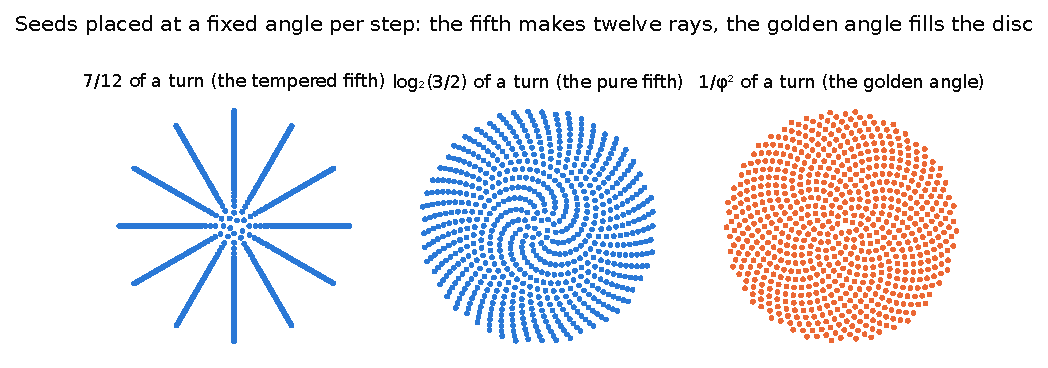
\includegraphics[width=0.95\textwidth]{golden-phyllotaxis}
  \caption{Seven hundred seeds at a fixed angle per step.}
  \label{fig:phyllo}
\end{figure}

\section{The shortest closed geodesic on the modular surface}

A hyperbolic element $\gamma\in\SL(2,\Z)$, one with $|\mathrm{tr}\,\gamma|>2$, has an axis in $\HH$.
That axis projects to a closed geodesic on the modular surface $\SL(2,\Z)\backslash\HH$ of length $2\,\mathrm{arccosh}(|\mathrm{tr}\,\gamma|/2)$.
The smallest such trace is 3, attained by $\gamma = \left(\begin{smallmatrix}2&1\\1&1\end{smallmatrix}\right)$.
Its axis joins its fixed points $-1/\varphi$ and $\varphi$, the roots of $z^2 - z - 1$.
The length is
\[
  2\,\mathrm{arccosh}\tfrac32 = 2\log\varphi^2 = 4\log\varphi = 1.9248\ldots
\]
So the shortest closed geodesic belongs to the golden ratio (Figure~\ref{fig:geodesic}).
In general the trace $t$ gives length $2\log\varepsilon_t$, where $\varepsilon_t = (t+\sqrt{t^2-4})/2$ is a unit of $\Q(\sqrt{t^2-4})$.
Traces $3,4,5,6$ give the fields $\Q(\sqrt5)$, $\Q(\sqrt3)$, $\Q(\sqrt{21})$ and $\Q(\sqrt2)$.
In Selberg's theory the closed geodesics play the role of the primes.
Their lengths enter the Selberg zeta function as the $\log p$ enter $\zeta$ (note~04), and they obey a prime geodesic theorem \cite{Iwaniec}.

\begin{figure}[ht]
  \centering
  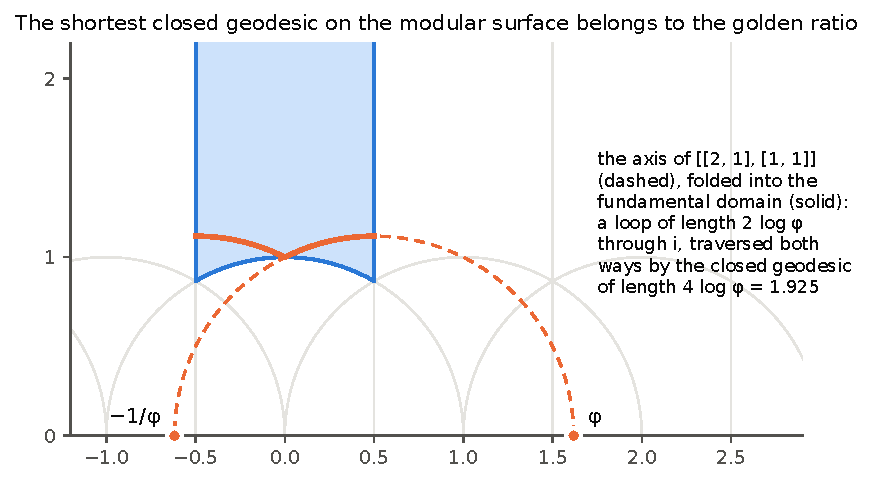
\includegraphics[width=0.8\textwidth]{golden-geodesic}
  \caption{The axis of $\left(\begin{smallmatrix}2&1\\1&1\end{smallmatrix}\right)$ (dashed), and the same geodesic folded into the fundamental domain (solid): a closed loop through $i$ of length $4\log\varphi$.}
  \label{fig:geodesic}
\end{figure}

\section{Level five: the icosahedron}

Reducing $\SL(2,\Z)$ modulo 5 gives $\mathrm{PSL}(2,\Z/5)$, a group of order 60.
Its elements have orders 1, 2, 3 and 5, in the numbers 1, 15, 20 and 24.
Those are the order statistics of $A_5$, the rotation group of the icosahedron.
The quotient $X(5) = \Gamma(5)\backslash\HH^*$ has 12 cusps, 30 images of $i$ and 20 images of $\rho$.
Since $12 - 30 + 20 = 2$, it is a sphere tiled as an icosahedron: the cusps are the vertices, the images of $i$ the edge midpoints, and the images of $\rho$ the face centres.
This is Klein's picture \cite{Klein}.
The vertices of a regular icosahedron can be taken to be the cyclic permutations of $(0,\pm1,\pm\varphi)$.
They lie on three golden rectangles (Figure~\ref{fig:ico}, left).
Here a twelve and the golden ratio do meet.
But these twelve are the $60/5$ cusps of $\Gamma(5)$, not the twelve tones of note~01.

\section{The golden ratio as a mass ratio}

Zamolodchikov showed that the Ising field theory in a magnetic field, at the critical temperature, has eight stable particles \cite{Zamolodchikov}.
Their masses are proportional to the Perron--Frobenius eigenvector of the $E_8$ Dynkin diagram.
The script computes that eigenvector (eigenvalue $2\cos\frac{\pi}{30}$, from the Coxeter number 30) and confirms all eight closed forms.
The first ratio is $m_2/m_1 = 2\cos\frac\pi5 = \varphi$.
Coldea and collaborators observed the two lowest modes in the quasi-one-dimensional Ising magnet CoNb$_2$O$_6$ by neutron scattering \cite{Coldea}.
Their ratio approaches $\varphi$ near the critical field (Figure~\ref{fig:ico}, right).
This is the clearest case of a number field, here $\Q(\sqrt5)$, setting a measured ratio of particle masses.

\begin{figure}[ht]
  \centering
  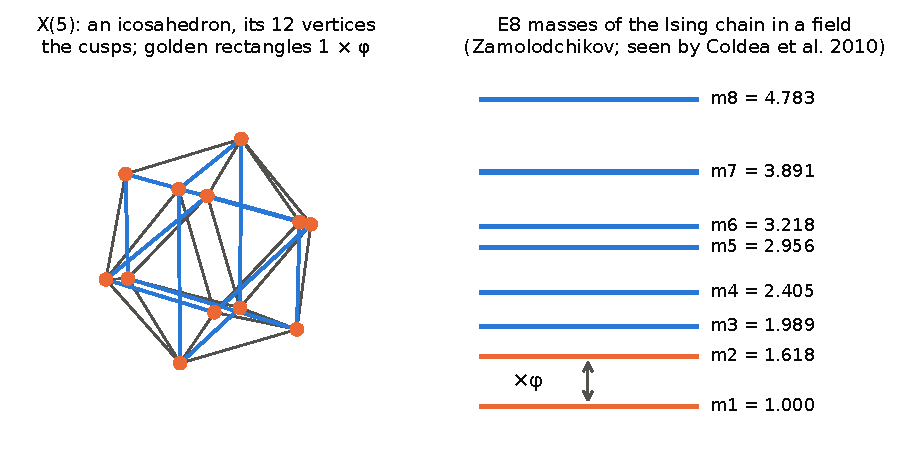
\includegraphics[width=0.92\textwidth]{golden-icosahedron-e8}
  \caption{Left: the icosahedron, with vertices $(0,\pm1,\pm\varphi)$ on three golden rectangles; for $X(5)$ these are the twelve cusps. Right: Zamolodchikov's $E_8$ masses.}
  \label{fig:ico}
\end{figure}

\section{Where the evidence stops}

The author's suggestion was that the golden ratio is how ``basically everything propagates, including matter''.
The evidence supports narrower statements.
$\varphi$ appears where five-fold or $E_8$ structure is present: phyllotaxis, icosahedral quasicrystals, and the $E_8$ Ising chain.
It also appears in the modular world at the shortest geodesic and at level five.
We found no evidence for the general claim.

\begin{question}
Is there a physical system whose spectrum is the length spectrum of closed geodesics on the modular surface, so that its lowest mode is $4\log\varphi$?
Does the level-five structure, the icosahedron $X(5)$, have a physical realisation tied to its modular forms, beyond its symmetry group?
\end{question}

\section*{Status of the statements}

\begin{center}
\small
\begin{tabular}{@{}p{0.62\textwidth}l@{}}
\toprule
Statement & Grade\\
\midrule
The twelve-tone symmetry is the Klein group, not $\varphi$ & \gradeLean{} (note 01)\\
Hurwitz; continued fractions of $\varphi$ and $\log_2\frac32$ & \gradeClassical, \gradeComputed\\
Golden angle and gap ratios in Vogel's model & \gradeComputed; physics \gradeClassical{} \cite{DouadyCouder}\\
Shortest closed geodesic $4\log\varphi$; minimal hyperbolic trace 3 & \gradeClassical, \gradeComputed\\
$\mathrm{PSL}(2,\Z/5)$ and $A_5$ order statistics; $X(5)$ an icosahedron & \gradeClassical, \gradeComputed\\
$E_8$ masses, $m_2/m_1=\varphi$; observed in CoNb$_2$O$_6$ & \gradeClassical, \gradeComputed\\
$\varphi$ governs propagation in general & not supported\\
The questions above & \gradeOpen\\
\bottomrule
\end{tabular}
\end{center}

\begin{thebibliography}{9}
\bibitem{Coldea} R.~Coldea et al., Quantum criticality in an Ising chain: experimental evidence for emergent $E_8$ symmetry, \emph{Science} 327 (2010), 177--180.
\bibitem{DouadyCouder} S.~Douady and Y.~Couder, Phyllotaxis as a physical self-organized growth process, \emph{Phys. Rev. Lett.} 68 (1992), 2098--2101.
\bibitem{Iwaniec} H.~Iwaniec, \emph{Spectral Methods of Automorphic Forms}, 2nd ed., American Mathematical Society, 2002.
\bibitem{Klein} F.~Klein, \emph{Vorlesungen \"uber das Ikosaeder}, Teubner, 1884.
\bibitem{Zamolodchikov} A.~B. Zamolodchikov, Integrals of motion and $S$-matrix of the (scaled) $T=T_c$ Ising model with magnetic field, \emph{Int. J. Mod. Phys. A} 4 (1989), 4235.
\end{thebibliography}

\end{document}
